\subsection{Question 1}
\subsubsection{Part A}

\newpage
\subsubsection{Part B}

\lstinputlisting[caption=Matlab Commands,showstringspaces=false,language=Matlab]{../lu_sym.m}

\subsubsection{Part C}
The complexity of Gauss elimination is is \(O(\frac{m^{3}}{3})\).
Regular gauss elimination works on an entire matrix ({\em i.e.,} touching all elements of the matrix) during \(LU\) factorization.
However, for a symmetric matrix we have proven in part A that we only need to touch the upper triangular elements of a matrix.
This constitutes half of the matrix.
Therefore, the complexity of the symmetric \(LU\) factorization algorithm will be \(\frac{1}{2}\frac{m^{3}}{3}\) or simply \(O(\frac{m^{3}}{6})\).

\newpage
\subsubsection{Part D}

\lstinputlisting[caption=Matlab Commands,showstringspaces=false,language=Matlab]{../q1_partD.m}
\lstinputlisting[caption=Matlab Commands,showstringspaces=false,language=Matlab]{../q1_partD_results}

It is clear from the results that the ratio between the run time of the symmetric \(LU\) factorization script over the Gauss elimination \(LU\) factorization script is converging to \(\frac{1}{2}\).
This confirms the complexity predicted for symmetric \(LU\) factorization in part C of this question.
Note, experiments were run on symmetric matrices with \(m \in \{30,40,50,60 \}\).

\newpage
\subsection{Question 2}

\subsubsection{Part A}
This code does the basic Gauss elimination \(LU\) factorization.
It is the same code used in question 1 during the comparison to the symmetric \(LU\) factorization.

\lstinputlisting[caption=Matlab Commands,showstringspaces=false,language=Matlab]{../lu_basic.m}

\subsubsection{Part B}
As stated in the question, we simply use Matlab's lu routine to accomplish this algorithm.
Note, Matlab's lu routine does partial pivoting.

\newpage
\subsubsection{Part C}

This code does complete pivoting before Gauss elimination.
The code returns [L,U,P,Q] where \(P\) and \(Q\) are permutation matrices.
The algorithm produces matrices for the equation \(PAQ = LU\). 

\lstinputlisting[caption=Matlab Commands,showstringspaces=false,language=Matlab]{../lu_pivot.m}

\subsubsection{Part D}


\newpage
\subsection{Question 3}
\subsubsection{Part A}
\subsubsection{Part B}
\subsubsection{Part C}
\subsubsection{Part D}




%\lstinputlisting[caption=Matlab Commands,showstringspaces=false,language=Matlab]{../find_vectors.m}


%\begin{figure}[th]
%  \centering
%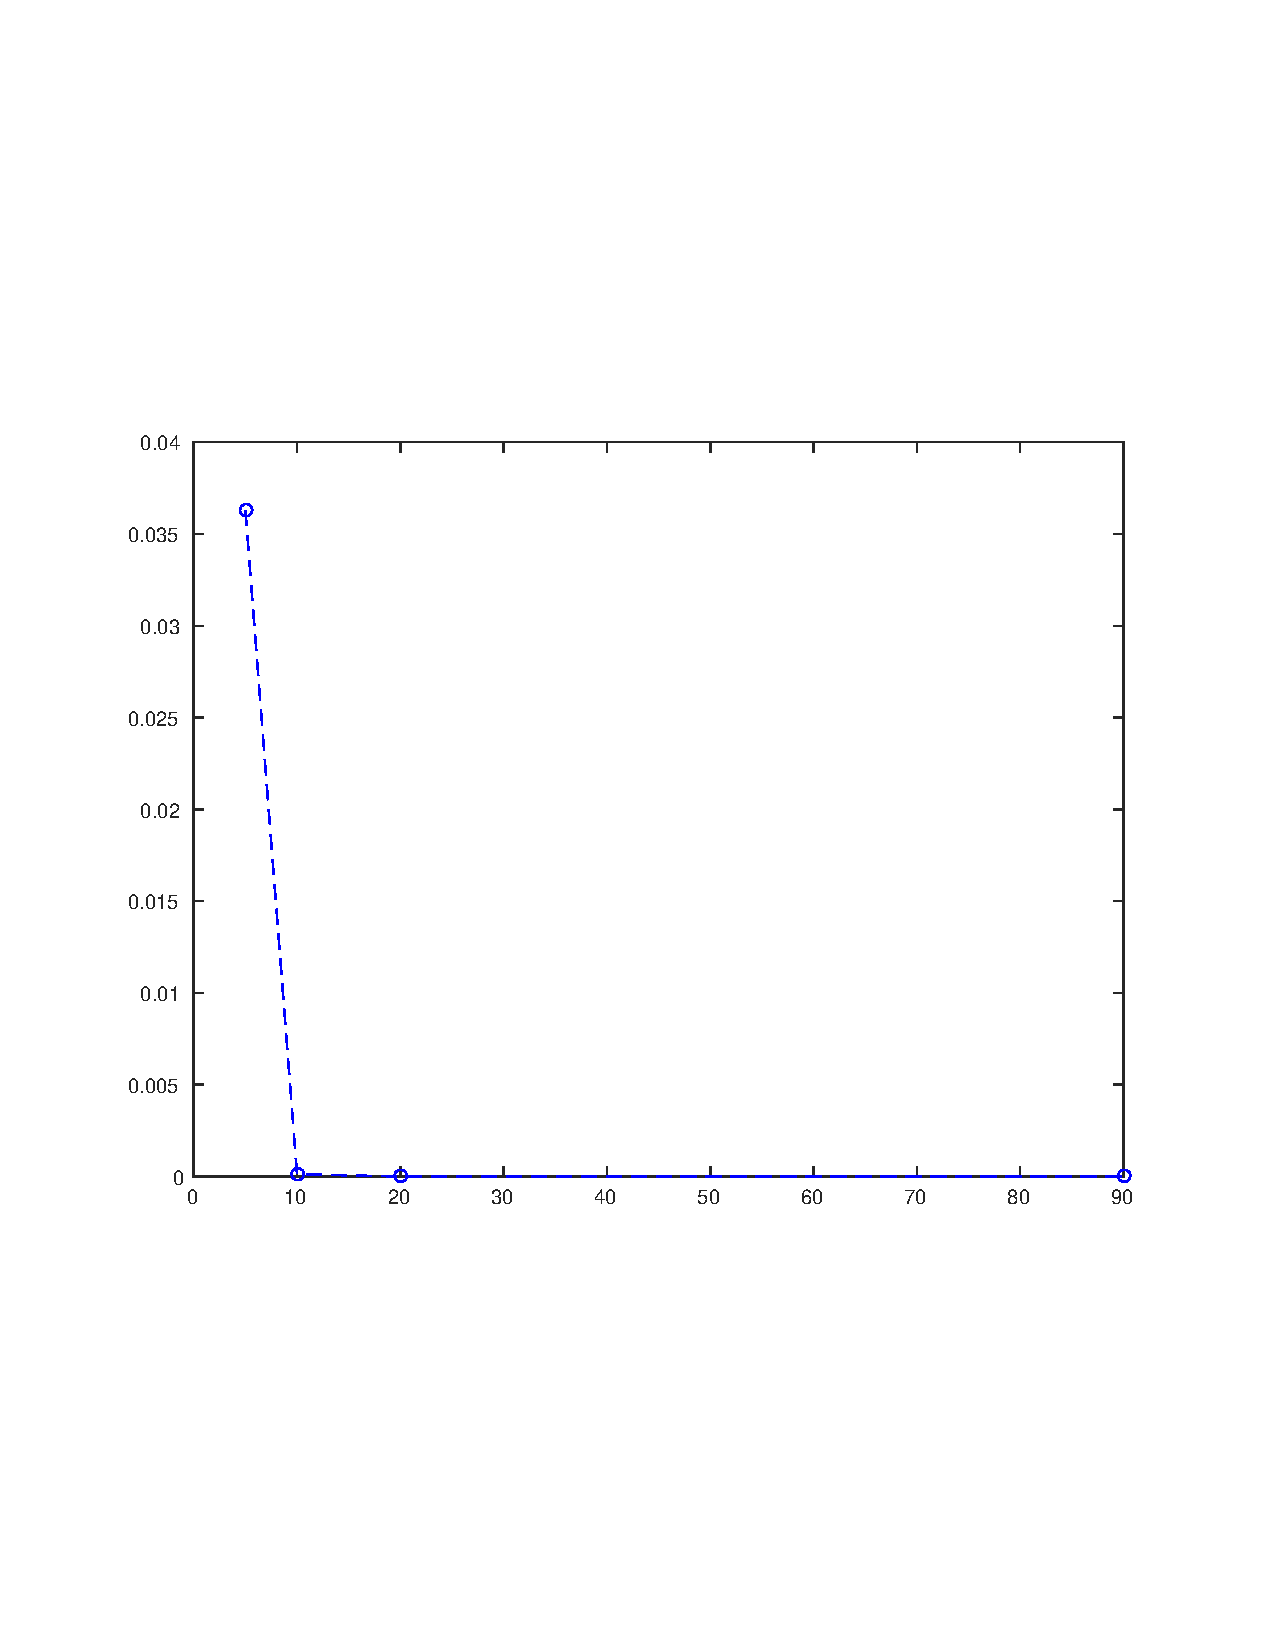
\includegraphics[trim=10mm 70mm 10mm 70mm, width=1.0\textwidth]{../q2_plots}
%\end{figure}
